% --------------------------------------------------------------
% This is all preamble stuff that you don't have to worry about.
% Head down to where it says "Start here"
% --------------------------------------------------------------
 
\documentclass[12pt]{article}
 
\usepackage[nouppercase,headsepline,footsepline,plainfootsepline]{scrpage2}
\automark{section}
\pagestyle{scrheadings}
%\clearscrheadfoot
\ihead{Numerical Sequences and Series}
%\ofoot[\pagemark]{\pagemark}% Optional argument controls chapter-starting pages
\ifoot[(Author)]{{\sl \hfill Meenmo K.}}

\usepackage[margin=1in]{geometry} 
\usepackage{amsmath,amsthm,amssymb,scrextend}
\usepackage{fancyhdr}
\usepackage{enumitem}
\usepackage{amsmath}
\usepackage{amssymb}
\usepackage{textcomp}
\usepackage{fancybox}
\usepackage{tikz}
\usepackage{cancel}
\usepackage{tasks}


\newcommand{\N}{\mathbb{N}}
\newcommand{\Z}{\mathbb{Z}}
\newcommand{\I}{\mathbb{I}}
\newcommand{\R}{\mathbb{R}}
\newcommand{\Q}{\mathbb{Q}}
\renewcommand{\qed}{\hfill$\blacksquare$}
\let\newproof\proof
\renewenvironment{proof}{\begin{addmargin}[1em]{0em}\begin{newproof}}{\end{newproof}\end{addmargin}\qed}
% \newcommand{\expl}[1]{\text{\hfill[#1]}$}
\setlength{\parindent}{0pt}
\newenvironment{theorem}[2][Theorem]{\begin{trivlist}
\item[\hskip \labelsep {\bfseries #1}\hskip \labelsep {\bfseries #2.}]}{\end{trivlist}}
\newenvironment{lemma}[2][Lemma]{\begin{trivlist}
\item[\hskip \labelsep {\bfseries #1}\hskip \labelsep {\bfseries #2.}]}{\end{trivlist}}
\newenvironment{problem}[2][Problem]{\begin{trivlist}
\item[\hskip \labelsep {\bfseries #1}\hskip \labelsep {\bfseries #2.}]}{\end{trivlist}}
\newenvironment{exercise}[2][Exercise]{\begin{trivlist}
\item[\hskip \labelsep {\bfseries #1}\hskip \labelsep {\bfseries #2.}]}{\end{trivlist}}
\newenvironment{reflection}[2][Reflection]{\begin{trivlist}
\item[\hskip \labelsep {\bfseries #1}\hskip \labelsep {\bfseries #2.}]}{\end{trivlist}}
\newenvironment{proposition}[2][Proposition]{\begin{trivlist}
\item[\hskip \labelsep {\bfseries #1}\hskip \labelsep {\bfseries #2.}]}{\end{trivlist}}
\newenvironment{corollary}[2][Corollary]{\begin{trivlist}
\item[\hskip \labelsep {\bfseries #1}\hskip \labelsep {\bfseries #2.}]}{\end{trivlist}}
 
 
\begin{document}
\section{Sequences of Real Numbers}
\subsection{Convergent Sequence}
\begin{block}A sequence is a map from $\mathbb{N}$ to a set. So a sequence of real numbers is a map $x\colon \mathbb{N}\to\mathbb{R}$ where we write $x_n=x(n), (x_n), \{x_n\}, \text{ or } x_1,x_2,...$.\end{block} \\

\begin{block}{\bf Definition} Let $(x_n)$ be a sequence in $\mathbb{R}\colon\; x\in\mathbb{R}$. We say $x_n$ converges to $x$ and write $x_n\to x$ or $\lim\limits_{n\to\infty} x_n = x$ if $\forall\;\epsilon>0, \exists\;N\in\mathbb{N}$ such that $\forall\;n\ge N,\; |x_n-x|<\epsilon$. Then we call $x$ the limit of $(x_n)$.\end{block}

\vspace{1.5\baselineskip}
\begin{block}{\bf Example} 
\begin{enumerate}[label=(\roman*)]
    \item Let $x_n=\frac{1}{n}.$ Show that $x_n\to 0$ as $n\to\infty$.
    \begin{itemize}
        \item Take $\epsilon>0$, and let $N>\frac{1}{\epsilon}$ such that $N\in \mathbb{N}.$
        \item Now, $\forall N\ge N,\; |x_n-0|=|x_n| = \frac{1}{n}\le \frac{1}{N}<\epsilon$.
    \end{itemize}
    
    \item Let $x_n = 1-\frac{1}{n^2}$. show that $x_n\to 1$ as $n\to \infty$.
    \begin{itemize}
        \item Take $\epsilon>0$, and let $N>\frac{1}{\epsilon}$ such that $N\in \mathbb{N}.$
        \item Now, $\forall N\ge N,\; |x_n- 1|=|1-\frac{1}{n^2} -1| = \frac{1}{n^2} \le \frac{1}{N^2} < \epsilon$.
    \end{itemize}
\end{enumerate}
\end{block}

\vspace{1.5\baselineskip}
\begin{block}{\bf Theorem} Let $(x_n)$ in $\mathbb{R}$ such that $x_n\to x$ and $x_n\to y$ then x=y.\end{block}

\vspace{1\baselineskip}
\begin{block}{\sl Proof.} 
\begin{itemize}
    \item Suppose by contradiction that $|x-y|>0$.
    \item Take $\epsilon=\frac{|x-y|}{2}$. Then
    \begin{itemize}
        \item $\exists\;N_1\in\mathbb{N}$ such that for $n\ge N_1,\;|x_n-x|<\epsilon$
        \item $\exists\;N_2\in\mathbb{N}$ such that for $n\ge N_2,\;|x_n-y|<\epsilon$
    \end{itemize}
    \item Let $N= \max(N_1,N_2)$, then $\forall\;n\geN$,
    $$0<|x-y| = |x-x_n+x_n-y| \le |x-x_n|+|x_n-y|<2\epsilon = |x-y|$$
    This contradicts to the initial assumption that $|x-y|>0$.
\end{itemize}
\end{block}

\newpage
\begin{block}{\bf Theorem} (Algebra of Limits) Let $(x_n), (y_n)$ in $\mathbb{R},\; x_n\to x,\; y_n\to y$. Then
\begin{enumerate}[label=(\roman*)]
    \item $x_n+y_n \to x+y,\; cx_n\to cx\;\;\forall c\in\mathbb{R}$
    \item $x_n\times y_n \to xy$
    \item If $y_n$ with $y\neq 0\;\;\forall\;n\in\mathbb{N},\;$then $\frac{x_n}{y_n}\to \frac{x}{y}.$
\end{enumerate}
\end{block}

\vspace{1\baselineskip}
\begin{block}{\sl Proof.}
\begin{enumerate}[label=(\roman*)]
    \item Let $\epsilon >0$. Then 
    \begin{itemize}
        \item $\exists\;N_1\in\mathbb{N}$ such that $\forall\;n\ge N_1,\;|x_n-x|<\frac{\epsilon}{2}$
        \item $\exists\;N_2\in\mathbb{N}$ such that $\forall\;n\ge N_2,\;|y_n-y|<\frac{\epsilon}{2}$
    \end{itemize}
    Let $N=\max(N_1,N_2)$. Then 
    $$\forall\;n\geN,\;|x_n+y_n-(x+y)|\le |x_n-x|+|y_n-y|<\frac{\epsilon}{2}+\frac{\epsilon}{2}=\epsilon$$
    %\item Then $\forall\;n\ge N=\max(N_1,N_2),\;|$
    
    \item $x_ny_n - xy \to 0\;\Leftrightarrow\; x_ny_n\to xy$.
    \item 
\end{enumerate}
\end{block}

\vspace{1\baselineskip}
\begin{block}{\bf Definition} Monotone Sequence: A sequence $(x_n)$ is called
\begin{enumerate}[label=(\roman*)]
    \item {\sl Monotonically Increasing }  if $x_n\le x_{n+1},\;\forall\;n\in\mathbb{N}$
    \item {\sl Monotonically Decreasing }  if $x_n\ge x_{n+1},\;\forall\;n\in\mathbb{N}$
    \item {\sl Monotone } if either (i) or (ii)
    \item {\sl Bounded } if $\exists\;M>0$ such that $|x_n|\le M\;\;\forall\;n\in\mathbb{N}$.
\end{enumerate}

\vspace{1\baselineskip}
\begin{block}{\bf Theorem} Let $(x_n)$ be monotone. Then $(x_n)$ is convergent if and only if $(x_n)$ is bounded.\\

{\sl Proof.}
\begin{itemize}
    \item Suppose $(x_n)$ is bounded, $x_n\le x_{n+1}\;\;\forall\;n\in\mathbb{N}.$
    \item Then $E = \{x_n\;|\;n\in\mathbb{N} \}$ is non-empty and bounded.
    \item So $x=\sup E$ exists in $\mathbb{R}$.
    \item Let $\epsilon>0,$ then $\exists\;N\in\mathbb{N}$ such that $x-\epsilon<x_N\le x$.
    \item Now $x-\epsilon <x_N\le x_n\le x\;\;\forall\;n\ge N$ by monotonicity.
    \item Hence $\forall\;n\ge N,\;|x_n-x|<\epsilon.$
\end{itemize}
{\sl Note. }If a sequence is convergent, then it is bounded.
\end{block}
\end{block}

\newpage
\subsection{Subsequences}
\begin{block}{\bf Definition}\\ Let $(x_n)$ be a sequence. Suppose $(n_k)$ is a sequence in $\mathbb{N}$. Then $(x_{n_k})$ is a {\sl subsequence}.

\vspace{1\baselineskip}
{\bf Proposition}\\ Let $(x_n)$ be a sequence, then $x_n\to x$ if and only if $x_{n_k}\to x$ for all subsequences $(x_{n_k})$ of $(x_n).$

\vspace{1\baselineskip}
{\bf Example} $x_n=(-1)^n$
\begin{itemize}
    \item Let $n_k=2k$ for $k\in\mathbb{N}$. Then $x_{n_k}=1\;\;\forall\;k$, so $x_{n_k}\to 1$.
    \item Now let $n_j = 2_j+1,\;j\in\mathbb{N}$. Then $x_{n_j}\to -1$. 
    \item Hence $(x_n)$ does not converge. 
\end{itemize}

\subsection{Cauchy Sequences}
\textbf{Definition}\\
A sequence of real numbers $(x_n)$ converges to $x$ if 
$\forall\;\epsilon > 0\;\exists\;\N\in\mathbb{N}$ such that $\forall\; n \ge \mathbb{N}, \; |x_n - x| < \epsilon$.\\

\textbf{Theorem} (Bolzano-Weierstrass)\\
Any bounded sequence $(x_n)$ in $\mathbb{R}$ has a convergent subsequence.\\

{\sl Proof.}
$$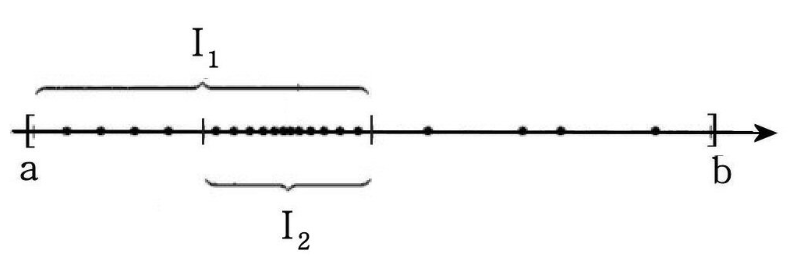
\includegraphics[height=2.7cm, width=13cm]{bolzano.png}$$
\begin{itemize}
    \item Suppose sequence $E = \{x_n\;|\; n \in \mathbb{N}\}$. 
    \item If $E$ is finite, then $\exists$ a subsequence $(x_{n_k})$ such that $x_{n_1}=x_{n_2}=x_{n_3}=\ldots=x_{n_k}=\ldots$ which is convergent.\\
    
    \item On the other hand, suppose $E$ is an infinite sequence.
    \item Now as $E$ is bounded, $\exists\;a<b\in\mathbb{R}$ such that $E\subset[a,b],$ and let $I_0=[a,b]$.
    \item Heine-Borel Theorem, $E$ has a limit point in $[a,b]\subset\mathbb{R}.$\\
    {\sl Recall that since $E$ is a closed and bounded $E$ is compact and has a limit point inside.}
    \item Let the limit point to be $x \in[a,b].$\\
    
    
    \item When $I_0$ is equally divided into two parts, infinitely many $x_n$ must be contained in, at least, one of two parts. Let us call it $I_1$.
    \item Reapting this steps, and we obtain $I_0,I_1,I_2,...\qquad$ i.e. $I_0\supset I_1\supset I_2\supset \ldots$
    
    \item Then choose $n_1\in I_1$, $n_2\in I_2$ such that $n_1<n_2$, $n_3\in I_3$ such that $n_1<n_2<n_3,\;\ldots$
    \item Then $\{x_{n_k}\}$ is a subsequence of $\{x_n\}$, and $x_{n_k}$ and the limit point $x$ are also contained in $I_k$.
    \item Thus we can derive that 
    $$|x_{n_k}-x| < \frac{M}{2^k}$$
    where $M = \frac{b-a}{2}$, so $\frac{M}{2^k}$ is the length of $I_k$.
    \item Since $\lim\limits_{n\to\infty} \frac{M}{2^n} = 0$, this implies that $\lim\limits_{k\to\infty} x_{n_k} = x$
\end{itemize}\\

\vspace{1\baselineskip}
\textbf{Definition}\\
A sequence $(x_n)$ in $\mathbb{R}$ is \textbf{Cauchy} if $\forall\;\epsilon > 0,\; \exists \; N \in \mathbb{N}$ such that $\forall\;n,m \ge \mathbb{N}|,\; |x_n - x_m| < \epsilon$.\\

{\sl Remark.} Cauchy does not require a \underline{known} limit point.\\

\vspace{1\baselineskip}
\textbf{Theorem} $(x_n)$ converges if and only if it is Cauchy.\\

{\sl Proof.}
\begin{itemize}
    \item $\Rightarrow$ Suppose $(x_n)$ converges, $x_n \rightarrow x$. 
    \item Let $\epsilon > 0$. Then $\exists\; N \in \mathbb{N}$ such that $\forall\;n\ge N,\; |x_n - x| < \frac{\epsilon}{2}.$
    \item Now if $n,m \ge N,\; |x_n - x_m| \le |x_n-x|+|x-x_m| < \epsilon.$\\
    
    \item $\Leftarrow$ Suppose $(x_n)$ is Cauchy.
    \item Step 1: $(x_N)$ is bounded.
    \begin{itemize}
        \item $\exists\; n \in \mathbb{N}$, such that $\forall\;n,m \ge N, |x_n-x_m|<1$.
        \item Thus $\forall\;n\ge N,\; |x_n| \le max(|x_n| +1, |x_1|,...,|x_N|)\le M\in\mathbb{R}$. \hfiill i.e. $(x_n)$ is bounded.
    \end{itemize}
    
    \item Step 2: Find the limit.
    \begin{itemize}
        \item By Bolzano-Weierstrass, $\exists$ a subsequence $(x_{n_k})$ such that $(x_{n_k}) \rightarrow x \in \mathbb{R}$.
        \item Let $\epsilon > 0$. Take $N_1 \in \mathbb{N}$ such that $\forall\; k\ge N_1,\; |x_{n_k} - x| <\frac{\epsilon}{2}.$
        \item Then $\exists\; N_2 > n_{N_1}$ such that $\forall\; n,m \ge N_2,\; |x_n -x_m| <\frac{\epsilon}{2}.$
        \item Now if $n \ge N_2,\; |x_n -x| \le |x_n -x_{n_{N_2}}| + |x_{n_{N_2}} - x|$ as $n_{N_2}\ge N_2 > N_1.$
    \end{itemize}
\end{itemize}



\textbf{Theorem}
\begin{enumerate}[label=(\roman*)]
    \item $\forall\;p>0, \frac{1}{n^p} \rightarrow 0$ as $n \rightarrow \infty$.
    \item $\forall\;x>0, x^{\frac{1}{n}} \rightarrow 1$ as $n \rightarrow \infty$.
    \item $n^{\frac{1}{n}} \rightarrow 1$ as $n \rightarrow \infty$.
    \item $\forall\; p\in \mathbb{R}, x>0, \frac{n^p}{(1+x)^n} \rightarrow 0$.
    \item If $0<x<1, x^n \rightarrow 0$ as $n \rightarrow \infty$.
\end{enumerate}

{\sl Proof.}
\begin{enumerate}[label=(\roman*)]
    \item Exercise
    \item 
    \begin{itemize}
        \item Suppose $x>1$.
        \item By the binomial theorem = $(1+x_n)^n \ge 1+nx_n$.
        \item So $0 < x_n < \frac{x-1}{n} \rightarrow 0$ as $n\rightarrow \infty$.
        \item Hence $x+n \rightarrow 0$. i.e. $x^{\frac{1}{n}} \rightarrow 1$.
        \item In the case(?) $0<x<1, \frac{1}{2} > 1,$ so $\frac{1}{x}^{\frac{1}{n}} \rightarrow 1$.
        \item So $x^{\frac{1}{n}} = \frac{1}{\frac{1}{2}^{\frac{1}{n}}} \rightarrow \frac{1}{1} = 1$
    \end{itemize}

    \item 
    \begin{itemize}
        \item Let $x_n = n^{\frac{1}{n}} -1 \ge 0$
        \item Then $n = (1+x_n)^n \ge \frac{n(n-1)}{2}x_n^2$.
        \hfill (if approach like (ii) not $\to 0$)
        \item So $0 \le x_n \le \sqrt{\frac{2}{n-1}}$ for $n\ge 2$.
    \end{itemize}
    
    
    \item 
    \begin{itemize}
        \item Let $p \in \mathbb{R}, x>0$.
        \item Take $k \in \mathbb{N}$ such that $k > p$.
        \item Suppose $n > 2k$.
        \item Then $(1+x)^n \ge \binom{n}k x^k = \frac{n(n-1)\ldots(n-k+1)}{k!} \ge \frac{n^k}{2^k k!} x^k.$
        \item So $0< \frac{n^p}{(1+x)^n} \le \frac{2^k k!}{x^k} n^{p-k} \rightarrow 0$. 
        \hfill ($p-k<0$ as $k>p$)
    \end{itemize}
    
    
    \item $0<x<1$.
    \begin{itemize}
        \item So $\frac{1}{(1+x)^n} \rightarrow 0$ by (iv). (choose p=0).
        \hfill (where $1+x$ is an arbitrary number)
        \item If $x \in (0,1), \exits\; y>0$ such that $x = \frac{1}{1+y}$.
        \item So $x^n = \frac{1}{(1+y)^n} \rightarrow 0$.
    \end{itemize}
\end{enumerate}

\newpage
\section{Sequence in a metric space}\\
\textbf{Definition}\\
Let $(X,d)$ be a metric space, $(x_n)$ a sequence in $X, x \in X$. We say $(x_n)$ converges to x if $\forall\;\epsilon > 0, \exists\;N\in \mathbb{N}$ such that  for all $n\ge N, d(x_n,x) < \epsilon$. We note $x_n \rightarrow x,$ or $\lim_{n\rightarrow \infty} x_n = x$ or.\\

\vspace{1\baselineskip}
\textbf{Example}
\begin{enumerate}[label=(\roman*)]
    \item In $\mathbb{R}, however, \frac{1}{n} \rightarrow 0$.
    
    \item In $(0,\infty),\; \frac{1}{n}$ does not converge.
\end{enumerate}
 
\vspace{1\baselineskip}
\textbf{Theorem}\\
 Let $(X,d)$ be a metric space, $(x_n) \subset X.$
 \begin{enumerate}[label=(\roman*)]
     \item  $x_n \rightarrow x$ iff every neighborhood of $x$ contains all, but finitely many of the terms $x_n$.
     \begin{itemize}
         \item $x_n = (-1)^n.\;b_1(1)$ contains infinitely many $x_n$.
         \item $x_n$ does not converge to 1.
     \end{itemize}
     \item If $x\in X, y\in X, x_n \rightarrow x, x_n\rightarrow y, $then $x=y$.
     \item If $(x_n)$ converges, it is bounded.
     \item If $\E \subset X$ and $x$ is a limit point of $E$, then $\exists$ a sequence in $(x_n) \subset E$ such that $x_n \rightarrow x$.
 \end{enumerate}
 
 \vspace{1\baselineskip}
 \textbf{Example}
 \begin{itemize}
     \item Take $(\mathbb{R}, d_{disc}).$
$$
 d_{disc}(x,y) =
 \begin{cases}
 1 \text{ if } x \neq y\\
 0 \text{ if } x = y
 \end{cases}
 \hfill (disc \text{ refers to discrete})$$
 
 \item Consider $x_n = \frac{1}{n}.$
 \item Note $d(x_n,0) = 1\;\; \forall\; n$ . So $\{{x_n}\} \subset B_2(0);$ hence ($x_n$) is bounded. 
 \item But if $x\in \mathbb{R}, $ eventually, $x_n \neq x\;\; \forall\; n$
 \hfill (all $x$ are distinct)
 \item so ($d(x_n, x) = 1 \;\;\forall\;n.$ 
 \item So $x_n \nrightarrow x\;\;\forall\;x\in\mathbb{R}$\hfill
 i.e. It does not converge.
 \end{itemize}
 
  


\end{block}

\end{document}